\documentclass[french,a4paper]{article}
\usepackage{lmodern}
\usepackage{amssymb,amsmath}
\usepackage{ifxetex,ifluatex}
\usepackage{fixltx2e} % provides \textsubscript
\ifnum 0\ifxetex 1\fi\ifluatex 1\fi=0 % if pdftex
  \usepackage[T1]{fontenc}
  \usepackage[utf8]{inputenc}
\else % if luatex or xelatex
  \ifxetex
    \usepackage{mathspec}
  \else
    \usepackage{fontspec}
  \fi
  \defaultfontfeatures{Ligatures=TeX,Scale=MatchLowercase}
\fi
% use upquote if available, for straight quotes in verbatim environments
\IfFileExists{upquote.sty}{\usepackage{upquote}}{}
% use microtype if available
\IfFileExists{microtype.sty}{%
\usepackage{microtype}
\UseMicrotypeSet[protrusion]{basicmath} % disable protrusion for tt fonts
}{}
\usepackage[top=2.4cm, bottom=2.1cm, outer=2cm, inner=4cm, headheight=40pt]{geometry}
\usepackage{hyperref}
\hypersetup{unicode=true,
            pdftitle={Formation aux GLM et aux modèles de distribution d'espèces},
            pdfauthor={Sébastien Rochette},
            pdfborder={0 0 0},
            breaklinks=true}
\urlstyle{same}  % don't use monospace font for urls
\ifnum 0\ifxetex 1\fi\ifluatex 1\fi=0 % if pdftex
  \usepackage[shorthands=off,main=french]{babel}
\else
  \usepackage{polyglossia}
  \setmainlanguage[]{french}
\fi
\usepackage{color}
\usepackage{fancyvrb}
\newcommand{\VerbBar}{|}
\newcommand{\VERB}{\Verb[commandchars=\\\{\}]}
\DefineVerbatimEnvironment{Highlighting}{Verbatim}{commandchars=\\\{\}}
% Add ',fontsize=\small' for more characters per line
\usepackage{framed}
\definecolor{shadecolor}{RGB}{248,248,248}
\newenvironment{Shaded}{\begin{snugshade}}{\end{snugshade}}
\newcommand{\KeywordTok}[1]{\textcolor[rgb]{0.13,0.29,0.53}{\textbf{#1}}}
\newcommand{\DataTypeTok}[1]{\textcolor[rgb]{0.13,0.29,0.53}{#1}}
\newcommand{\DecValTok}[1]{\textcolor[rgb]{0.00,0.00,0.81}{#1}}
\newcommand{\BaseNTok}[1]{\textcolor[rgb]{0.00,0.00,0.81}{#1}}
\newcommand{\FloatTok}[1]{\textcolor[rgb]{0.00,0.00,0.81}{#1}}
\newcommand{\ConstantTok}[1]{\textcolor[rgb]{0.00,0.00,0.00}{#1}}
\newcommand{\CharTok}[1]{\textcolor[rgb]{0.31,0.60,0.02}{#1}}
\newcommand{\SpecialCharTok}[1]{\textcolor[rgb]{0.00,0.00,0.00}{#1}}
\newcommand{\StringTok}[1]{\textcolor[rgb]{0.31,0.60,0.02}{#1}}
\newcommand{\VerbatimStringTok}[1]{\textcolor[rgb]{0.31,0.60,0.02}{#1}}
\newcommand{\SpecialStringTok}[1]{\textcolor[rgb]{0.31,0.60,0.02}{#1}}
\newcommand{\ImportTok}[1]{#1}
\newcommand{\CommentTok}[1]{\textcolor[rgb]{0.56,0.35,0.01}{\textit{#1}}}
\newcommand{\DocumentationTok}[1]{\textcolor[rgb]{0.56,0.35,0.01}{\textbf{\textit{#1}}}}
\newcommand{\AnnotationTok}[1]{\textcolor[rgb]{0.56,0.35,0.01}{\textbf{\textit{#1}}}}
\newcommand{\CommentVarTok}[1]{\textcolor[rgb]{0.56,0.35,0.01}{\textbf{\textit{#1}}}}
\newcommand{\OtherTok}[1]{\textcolor[rgb]{0.56,0.35,0.01}{#1}}
\newcommand{\FunctionTok}[1]{\textcolor[rgb]{0.00,0.00,0.00}{#1}}
\newcommand{\VariableTok}[1]{\textcolor[rgb]{0.00,0.00,0.00}{#1}}
\newcommand{\ControlFlowTok}[1]{\textcolor[rgb]{0.13,0.29,0.53}{\textbf{#1}}}
\newcommand{\OperatorTok}[1]{\textcolor[rgb]{0.81,0.36,0.00}{\textbf{#1}}}
\newcommand{\BuiltInTok}[1]{#1}
\newcommand{\ExtensionTok}[1]{#1}
\newcommand{\PreprocessorTok}[1]{\textcolor[rgb]{0.56,0.35,0.01}{\textit{#1}}}
\newcommand{\AttributeTok}[1]{\textcolor[rgb]{0.77,0.63,0.00}{#1}}
\newcommand{\RegionMarkerTok}[1]{#1}
\newcommand{\InformationTok}[1]{\textcolor[rgb]{0.56,0.35,0.01}{\textbf{\textit{#1}}}}
\newcommand{\WarningTok}[1]{\textcolor[rgb]{0.56,0.35,0.01}{\textbf{\textit{#1}}}}
\newcommand{\AlertTok}[1]{\textcolor[rgb]{0.94,0.16,0.16}{#1}}
\newcommand{\ErrorTok}[1]{\textcolor[rgb]{0.64,0.00,0.00}{\textbf{#1}}}
\newcommand{\NormalTok}[1]{#1}
\usepackage{longtable,booktabs}
\usepackage{graphicx,grffile}
\makeatletter
\def\maxwidth{\ifdim\Gin@nat@width>\linewidth\linewidth\else\Gin@nat@width\fi}
\def\maxheight{\ifdim\Gin@nat@height>\textheight\textheight\else\Gin@nat@height\fi}
\makeatother
% Scale images if necessary, so that they will not overflow the page
% margins by default, and it is still possible to overwrite the defaults
% using explicit options in \includegraphics[width, height, ...]{}
\setkeys{Gin}{width=\maxwidth,height=\maxheight,keepaspectratio}
\IfFileExists{parskip.sty}{%
\usepackage{parskip}
}{% else
\setlength{\parindent}{0pt}
\setlength{\parskip}{6pt plus 2pt minus 1pt}
}
\setlength{\emergencystretch}{3em}  % prevent overfull lines
\providecommand{\tightlist}{%
  \setlength{\itemsep}{0pt}\setlength{\parskip}{0pt}}
\setcounter{secnumdepth}{5}
% Redefines (sub)paragraphs to behave more like sections
\ifx\paragraph\undefined\else
\let\oldparagraph\paragraph
\renewcommand{\paragraph}[1]{\oldparagraph{#1}\mbox{}}
\fi
\ifx\subparagraph\undefined\else
\let\oldsubparagraph\subparagraph
\renewcommand{\subparagraph}[1]{\oldsubparagraph{#1}\mbox{}}
\fi

%%% Use protect on footnotes to avoid problems with footnotes in titles
\let\rmarkdownfootnote\footnote%
\def\footnote{\protect\rmarkdownfootnote}

%%% Change title format to be more compact
\usepackage{titling}

% Create subtitle command for use in maketitle
\newcommand{\subtitle}[1]{
  \posttitle{
    \begin{center}\large#1\end{center}
    }
}

\setlength{\droptitle}{-2em}
  \title{Formation aux GLM et aux modèles de distribution d'espèces}
  \pretitle{\vspace{\droptitle}\centering\huge}
  \posttitle{\par}
  \author{Sébastien Rochette}
  \preauthor{\centering\large\emph}
  \postauthor{\par}
  \predate{\centering\large\emph}
  \postdate{\par}
  \date{14 mars, 2018}

% GIS and R Course
% author : Sébastien Rochette
% contact : sebastienrochettefr@gmail.com
% website : http://statnmap.com

% \documentclass[a4paper]{article}
% Lang EN = 1, FR = 2
% \def\Lang{\Sexpr{Lang}} % 
% -- Command to find which language is loaded in babel -- %
% http://tex.stackexchange.com/questions/287667/ifpackagewith-doesnt-behave-as-i-expected-with-global-options
\usepackage{xparse}
\ExplSyntaxOn
\NewDocumentCommand{\packageoptionsTF}{mmmm}
 {
  \stanton_package_options:nnTF { #1 } { #2 } { #3 } { #4 }
 }

\cs_new_protected:Nn \stanton_package_options:nnTF
 {
  \clist_map_inline:nn { #2 }
   {
    \clist_if_in:cnTF { opt@#1.sty } { ##1 }
     { #3 } % it's a local option
     {
      \clist_if_in:cnTF { @classoptionslist } { ##1 }
       { #3 } % it's a global option
       { #4 }
     }
   }
}
\ExplSyntaxOff

% -- Define a variable depending on language -- %
\newcommand{\Lang}{0}

\makeatletter
\@ifpackageloaded{babel}{
  \packageoptionsTF{babel}{english}{%
    \renewcommand{\Lang}{1}% english
  }{%
    \renewcommand{\Lang}{2}% french
  }
}{}
\makeatother

% -- Define specific lateX options depending on language -- %
\ifnum\Lang = 1
  % \usepackage[english]{babel}
  \usepackage{enumitem}
  \setlist{itemsep = 0pt}
  \setlist{topsep = 0pt}
\fi
\ifnum\Lang = 2
  % \usepackage[french]{babel}
\fi

% --
\usepackage[utf8]{inputenc}
\usepackage[T1]{fontenc}
\usepackage{amsmath}
%\usepackage{amssymb,amsfonts,textcomp}
\usepackage{color}
\usepackage{array}
\usepackage{hhline}
%\usepackage[linktocpage=true]{hyperref} % to have only number clickable in toc
\hypersetup{linktocpage=true, colorlinks=true, linkcolor=[RGB]{241,85,34}, citecolor=[RGB]{241,85,34}, filecolor=[RGB]{241,85,34}, urlcolor=[RGB]{241,85,34}}
%\usepackage[pdftex]{graphicx}
\usepackage{tikz}
%\usepackage{float} % To force figure to be placed where I want with H
% do not use float as it changes space between figures and their caption.
% Better use [!h] option for figures
\usepackage[normalem]{ulem} % to underline text on multiple lines

\renewcommand{\emph}[1]{\textit{#1}}

\usepackage{lmodern} % For higher definition fonts
\usepackage[font = footnotesize, labelfont = bf, margin = 1cm]{caption} %name=Fig.

% Text styles
\newcommand\textstyleInternetlink[1]{\textcolor[RGB]{21,183,214}{#1}}
\newcommand\Greytext[1]{\textcolor[RGB]{75,75,75}{#1}}
\newcommand\LightGrey[1]{\textcolor[RGB]{173,169,174}{#1}}
\newcommand\OtherGrey[1]{\textcolor[RGB]{200,200,200}{#1}}


% List styles
%\newcommand\liststyleWWviiiNumii{%
%\renewcommand\labelitemi{{\textbullet}}
%\renewcommand\labelitemii{{\textbullet}}
%\renewcommand\labelitemiii{{\textbullet}}
%\renewcommand\labelitemiv{{\textbullet}}
%}

\AtBeginDocument{
\def\labelitemi{$\bullet$}%
\def\labelitemii{$\circ$}%
\def\labelitemiii{$-$}%
\def\labelitemiv{$-$}%
}

% FIGURES
% \graphicspath{{/mnt/Data/Formation_SIG-et-R/00_Original_TD_support/img_QGIS/}{/mnt/Data/Formation_SIG-et-R/00_Original_TD_support/figureR/}{/mnt/Data/Formation_SIG-et-R/00_Original_TD_support/Figures_Pres/}{/mnt/Data/autoentrepreneur/Presentation_Produits/SRochettePresentation-img/}}

%\setlength{\abovecaptionskip}{5pt}
%\setlength{\belowcaptionskip}{10pt}


% DIMENSIONS - MARGINS
% \usepackage[top=2.4cm, bottom=2.1cm, outer=2cm, inner=4cm, headheight=40pt]{geometry} %heightrounded
%\setlength\hoffset{0cm}
%\setlength\voffset{0cm}
\setlength\topmargin{-2cm}
%\setlength\headheight{2cm}
\setlength\headsep{0.50cm}
%\setlength\textheight{25.7cm}
\setlength\footskip{1.1cm}
\setlength{\parindent}{0em}
%\setlength{\parskip}{0em}
\setlength\belowcaptionskip{5pt}
\setlength\abovecaptionskip{8pt}
%\let\oldfigure\figure
%\let\oldtable\table
%\def\figure{\setlength\abovecaptionskip{5pt}\oldfigure}
%\def\table{\setlength\belowcaptionskip{1cm}\oldtable}
%\usepackage{caption} %[font = small]
%\setlength{\abovecaptionskip}{10pt plus 5pt minus 5pt}
%\captionsetup[table]{skip = 10pt}
%\captionsetup[figure]{skip = 10pt}
%\setlength\longindentation 0.60\textwidth

% \usepackage{lastpage} % to calculate number of pages to put in footer
\usepackage{pageslts}

% ----------
% BACKGROUND
% ----------
\usepackage{eso-pic}
\newcommand\BackgroundPic{%
\put(0,0){%
\parbox[b][\paperheight]{\paperwidth}{%
\vfill
\centering
  \includegraphics[width=\paperwidth,height=\paperheight]{Background_light_topdown_ThinkR.png}%
\vfill
}}}
\newcommand\BackgroundPicTitle{%
\put(0,0){%
\parbox[b][\paperheight]{\paperwidth}{%
\vfill
\centering
  \includegraphics[width=\paperwidth,height=\paperheight]{Background_Title_light_ThinkR.png}%
\vfill
}}}

%...and this immediately after \begin{document}:
%\AddToShipoutPicture*{\BackgroundPic}
%The * will make sure that the background picture will only be put on one page.
%If you wish to use the picture on multiple pages, skip the *:
%\AddToShipoutPicture{\BackgroundPic}
%Then use this command to stop using the background picture:
%\ClearShipoutPicture


% ----------
% MISE EN FORME DES TITRES
% ----------
%\renewcommand{\thesection}{\arabic{section}}
%\renewcommand{\thesubsection}{\arabic{section}.\arabic{subsection}}
%\renewcommand{\thesubsubsection}{\arabic{section}.\arabic{subsection}.\arabic{subsubsection}}

%% Provide a definition to \subparagraph to keep titlesec happy
\let\subparagraph\oldsubparagraph
\let\paragraph\oldparagraph
%% Load titlesec
%\usepackage[compact]{titlesec}
\usepackage{titlesec}
%% Revert \subparagraph to the Rmd definition
% Redefines (sub)paragraphs to behave more like sections
\ifx\paragraph\undefined\else
\let\oldparagraph\paragraph
\renewcommand{\paragraph}[1]{\oldparagraph{#1}\mbox{}}
\fi
\ifx\subparagraph\undefined\else
\let\oldsubparagraph\subparagraph
\renewcommand{\subparagraph}[1]{\oldsubparagraph{#1}\mbox{}}
\fi


%\titleformat{(command)}[(shape)]{(format)}{(label)}{(sep)}{(before)}[(after)]
\titleformat{\section}%
[block]% style du titre (block, hang, display, runin, leftmargin, drop, wrap)
{\Large\color[RGB]{21,183,214}}%changement de fonte commun au numéro et au titre
{\thesection.}% spécification du numéro
{1em}% 1em espace entre le numéro et le titre
{}% changement de fonte du titre

\titleformat{\subsection}%
[block]% style du titre (block, hang, display, runin, leftmargin, drop, wrap)
{\large\bfseries} %\itshape {\Large\bfseries\color[RGB]{30,115,190}}%changement de fonte commun au numéro et au titre
{\thesubsection.}% spécification du numéro
{1em}% {1em}% espace entre le numéro et le titre
{}% changement de fonte du titre

\titleformat{\subsubsection}%
[block]% style du titre (block, hang, display, runin, leftmargin, drop, wrap)
{\large} %\itshape {\Large\bfseries\color[RGB]{30,115,190}}%changement de fonte commun au numéro et au titre
{\thesubsubsection.}% spécification du numéro
{1em}% {1em}% espace entre le numéro et le titre
{}% changement de fonte du titre

\titleformat{\paragraph}%
[block]% style du titre (block, hang, display, runin, leftmargin, drop, wrap)
{\itshape} %\itshape {\Large\bfseries\color[RGB]{30,115,190}}%changement de fonte commun au numéro et au titre
{\theparagraph.}% spécification du numéro
{1em}% {1em}% espace entre le numéro et le titre
{}% changement de fonte du titre

\titleformat{\subparagraph}%
[block]% style du titre (block, hang, display, runin, leftmargin, drop, wrap)
{\itshape} %\itshape {\Large\bfseries\color[RGB]{30,115,190}}%changement de fonte commun au numéro et au titre
{\thesubparagraph.}% spécification du numéro
{1em}% {1em}% espace entre le numéro et le titre
{}% changement de fonte du titre


%\titlespacing*{(command)}{(left)}{(beforesep)}{(aftersep)}[(right)]
\titlespacing*{\section}{0em}{*4}{*1}

% A break for each new section with figures printed before new section
% \newcommand{\sectionbreak}{\clearpage}
% \newcommand{\sectionbreak}{\clearpage\phantomsection} % if hyperref loaded before titlesec

% Title numbering depth
\setcounter{secnumdepth}{4}
% Table of content depth
\setcounter{tocdepth}{3}
\renewcommand\contentsname{Content} % toc title


% -----------
% MISE EN FORME TEXTES SPECIAUX
% -----------
% Additionnal Text colors
\usepackage{xcolor}
\definecolor{backcolor}{RGB}{235, 235, 235}

\newcommand{\mybox}[1]{\par\noindent\colorbox{backcolor}
{\parbox{\dimexpr\textwidth-2\fboxsep\relax}{#1}}}

\newcommand{\keyword}[1]{\textcolor{red!60!black}{#1}}
\newcommand{\advert}[1]{\textit{\textcolor{orange!80!black}{#1}}}
\newcommand{\exo}[1]{\textit{\textcolor{green!80!black}{#1}}}
%\newcommand{\codecommand}[1]{\par\noindent\colorbox{backcolor}{\texttt{#1}}}
%\newcommand{\menucommand}[1]{\par\fontfamily{pcr}\fontsize{12}{12}\selectfont\color{red}\noindent\colorbox{shadecolor}{\textit{#1}}}{\par}
\newcommand{\menucommand}[1]{\textit{\textcolor{blue!80!black}{#1}}}
\newcommand{\codecommand}[1]{\texttt{\colorbox{backcolor}{#1}}}

\newenvironment{important}{\par\color{black!80!green}\itshape}{\par}

\newsavebox{\selvestebox}
\newenvironment{redbox}
  {
   \begin{lrbox}{\selvestebox}%
   \begin{minipage}{\dimexpr\columnwidth-2\fboxsep\relax}}
  {\end{minipage}\end{lrbox}%
   \colorbox[HTML]{FF7F7F}{\usebox{\selvestebox}}
   }

% \newsavebox{\selvestebox}
\newenvironment{codebox}{
  \begin{lrbox}{\selvestebox}%
}{
  \end{lrbox}%
  \colorbox{backcolor}{\usebox{\selvestebox}}
}

% - source: http://tex.stackexchange.com/questions/82028/how-do-i-create-a-variant-of-the-snugshade-box-from-the-framed-package-to-wrap-m
\newenvironment{blueShaded}[1][D6E8F5]{
  \definecolor{shadecolor}{HTML}{#1}%
  \begin{snugshade}%
}{%
    \end{snugshade}%
}

% -- command for pandoc trick with \begin and \end -- %
\newcommand{\nopandoc}[1]{#1}

% ----------
% Pour justifier le texte apres un alignement à gauche
% Utile pour le texte en caractère tt qui ne se coupe pas
% ----------
\usepackage{ragged2e}

% \input{/mnt/Data/ThinkR/Gitlab/vignette-thinkr/latex/MiseEnFormeTitreFormationRmd_NoSectionBreak.tex}

\ifnum\Lang = 1
% ---------------
% HEADER / FOOTER
% ---------------
\usepackage{fancyhdr}
\pagestyle{fancy}
%\fancyhf{}
\fancyhead[L]{
\hspace{-1cm}\LARGE{\textbf{\href{https://thinkr.fr/}{ThinkR}}}\\
%\hspace{-1cm}\normalsize{\Greytext{Modélisation statistique, analyse de données géographiques et cartographie}}\\
\hspace{-1cm}\normalsize{\Greytext{Courses and consulting for R}}\\
%\normalsize{\href{url:http://statnmap.com/}{\textstyleInternetlink{http://statnmap.com/}}}
}
\fancyhead[R]{\Greytext{\textit{Created on \today}\hspace{-1cm}}}
%
\fancyfoot[L]{\Greytext{\hspace{-1cm}Sébastien Rochette}}
\fancyfoot[C]{\href{mailto:sebastien@thinkr.fr}{sebastien@thinkr.fr}}
\fancyfoot[R]{\Greytext{\thepage\ / \pageref*{LastPage}\hspace{-1cm}}}
%\cfoot{Page \thepage\ (\theCurrentPage) of \lastpageref{LastPages}}
\renewcommand{\headrulewidth}{0pt}
\renewcommand{\footrulewidth}{0pt}
%\fancyheadoffset{length}


\fi
\ifnum\Lang = 2
% ---------------
% HEADER / FOOTER
% ---------------
\usepackage{fancyhdr}
\pagestyle{fancy}
%\fancyhf{}
\fancyhead[L]{
\hspace{-1cm}\LARGE{\textbf{\href{https://thinkr.fr/}{ThinkR}}}\\
%\hspace{-1cm}\normalsize{\Greytext{Modélisation statistique, analyse de données géographiques et cartographie}}\\
\hspace{-1cm}\normalsize{\Greytext{Formation et consultance sur R}}\\
%\normalsize{\href{url:http://sebrock.fr/}{\textstyleInternetlink{http://sebrock.fr/}}}
}
\fancyhead[R]{\Greytext{\textit{Créé le \today}\hspace{-1cm}}}
%
\fancyfoot[L]{\Greytext{\hspace{-1cm}Sébastien Rochette}}
\fancyfoot[C]{\href{mailto:sebastien@thinkr.fr}{sebastien@thinkr.fr}}
% \fancyfoot[R]{\Greytext{\thepage\ / \pageref*{LastPage}\hspace{-1cm}}}
%\cfoot{Page \thepage\ (\theCurrentPage) of \lastpageref{LastPages}}
\fancyfoot[R]{\Greytext{\thepage\ / \pageref*{LastPage}\hspace{-1cm}}}
\renewcommand{\headrulewidth}{0pt}
\renewcommand{\footrulewidth}{0pt}
%\fancyheadoffset{length}

\fi

% -- Graphic path -- %
% \graphicspath{{/mnt/Data/Formation_SIG-et-R/00_Original_TD_support/img_QGIS/}{/mnt/Data/Formation_SIG-et-R/00_Original_TD_support/figureR/}{/mnt/Data/Formation_SIG-et-R/00_Original_TD_support/Figures_Pres/}{/mnt/Data/autoentrepreneur/Presentation_Produits/SRochettePresentation-img/}}
\graphicspath{{/mnt/Data/ThinkR/Gitlab/vignette-thinkr/img/}}

% \title{GIS and R Course}
% \author{Sébastien Rochette}

\setcounter{section}{0} % Value for first section


\hypersetup{pdfauthor=Sébastien Rochette, pdftitle=Formation ThinkR, pdfsubject=Formation à R, pdfkeywords=R, pdfcreator=pdflatex}

%----------------------------------------------------------------------------------------
% TITLE PAGE
%----------------------------------------------------------------------------------------

\newcommand*{\titleGM}{\begingroup % Create the command for including the title page in the document
\hbox{ % Horizontal box
%\hspace*{0.2\textwidth} % Whitespace to the left of the title page
%\hspace*{0.2\textwidth}
\OtherGrey{\rule{1pt}{\textheight}} % Vertical line
\hspace*{0.05\textwidth} % Whitespace between the vertical line and title page text
\parbox[b]{0.75\textwidth}{ % Paragraph box which restricts text to less than the width of the page

{\noindent\Huge\bfseries\textstyleInternetlink{ Formation à R}}\\[2\baselineskip] % Title
{\large{Modélisation avec les GLM}}\\[4\baselineskip] % Tagline or further description
{\Large \textsc{Sébastien Rochette, ThinkR}} % Author name

\vspace{0.5\textheight} % Whitespace between the title block and the publisher
{\noindent \href{url:https://thinkr.fr}{ThinkR}}\\[\baselineskip] % Publisher and logo
}}
\endgroup}

\AtBeginDocument{\let\maketitle\relax}

\begin{document}
\maketitle

\pagenumbering{arabic}

%\bigskip
%\medskip

%\begin{center}
%\href{url:http://statnmap.com}{\textstyleInternetlink{\huge{Modelling distribution of species in the Bay of Biscay}}}\\
%\large{Sébastien Rochette}\\
%\end{center}
\setcounter{page}{0}
\pagestyle{empty} % Removes page numbers
\AddToShipoutPicture{\BackgroundPicTitle}

\titleGM

\pagebreak
\pagestyle{fancy}
% \clearpage\setcounter{page}{1}\pagestyle{Standard}
\AddToShipoutPicture{\BackgroundPic}

{
\setcounter{tocdepth}{2}
\tableofcontents
}
\section{Préface}\label{preface}

\emph{La version d'origine de cette formation a été créée par Olivier Le
Pape et Étienne Rivot à Agrocampus Ouest (Rennes, France). Depuis mon
doctorat dans leur équipe, je mets à jour constamment cette formation au
gré de ma recherche et de l'évolution du logiciel R.}

\begin{Shaded}
\begin{Highlighting}[]
  \CommentTok{# Generated with R and rmarkdown: Roadmap version - Students}
\end{Highlighting}
\end{Shaded}

\section{Présentation de l'étude}\label{presentation-de-letude}

\textbf{\advert{Le contexte et les objectifs de votre étude définissent le type de modélisation que vous allez mettre en place sur votre jeu de données.}\\
Ici, nous utilisons les modèles linéaires généralisés pour produire une
carte de distribution moyenne de la nourricerie de soles communes de la
baie de Vilaine}.

\subsection{Contexte}\label{contexte}

\begin{itemize}
\tightlist
\item
  Les zones côtières et les estuaires sont des habitats halieutiques
  essentiels

  \begin{itemize}
  \tightlist
  \item
    Zones à forte production
  \item
    Nourriceries
  \item
    Zones restreintes avec de fortes densités (Fig.
    \ref{fig:figPlaiceBox})
  \end{itemize}
\end{itemize}



\begin{figure}[!h]

{\centering 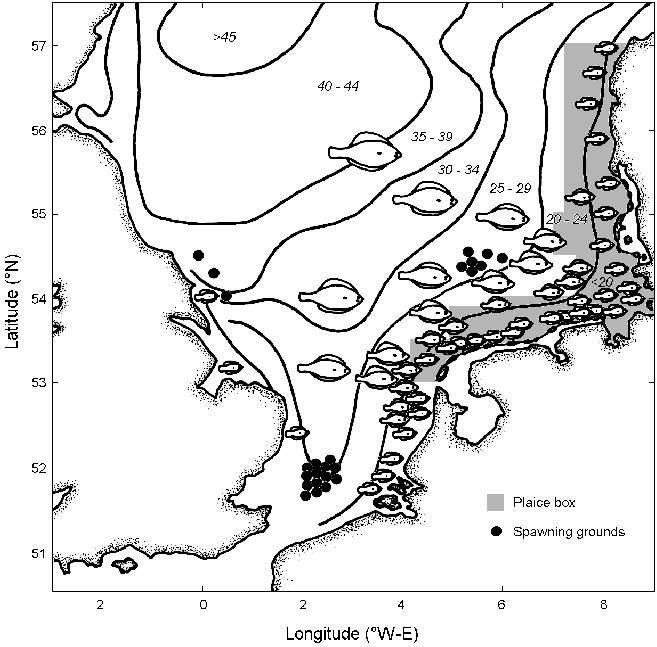
\includegraphics[width=0.5\linewidth]{/mnt/Data/ThinkR/Gitlab/formation-glm/03_Figures/00_Presentation/PlaiceBox_crop} 

}

\caption{Plaice box (Rijnsdorp \emph{et al.})}\label{fig:figPlaiceBox}
\end{figure}

\begin{itemize}
\tightlist
\item
  Pression anthropique élevée

  \begin{itemize}
  \tightlist
  \item
    Perte de surface disponibles (Fig. \ref{fig:figHighPressure}a)
  \item
    Qualité des habitats alterée (Fig. \ref{fig:figHighPressure}b)
  \end{itemize}
\end{itemize}




\begin{itemize}
\tightlist
\item
  Impact sur le renouvellement des populations

  \begin{itemize}
  \tightlist
  \item
    Jeune stades = Gouleau d'étranglement
  \item
    La taille et la qualité des nourriceries côtières influent sur la
    production de juvéniles
  \end{itemize}
\end{itemize}

\begin{figure}[!h]

{\centering 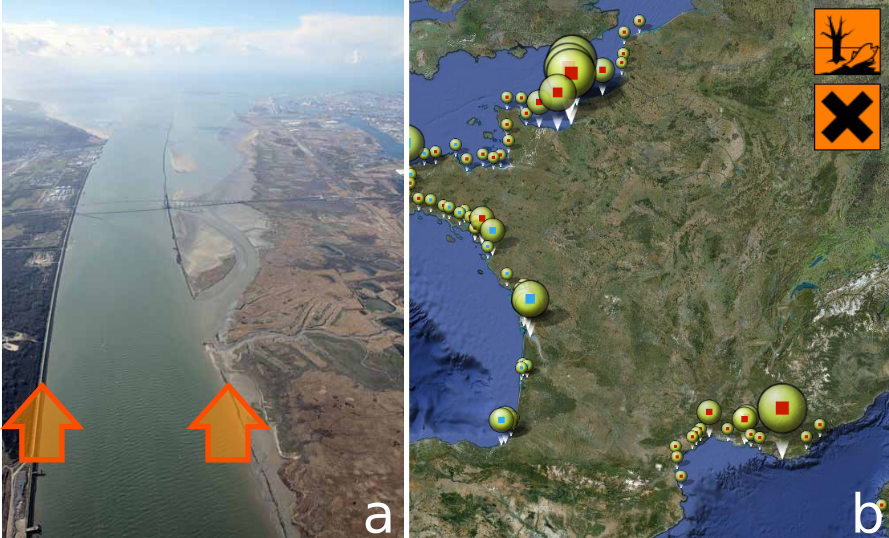
\includegraphics[width=0.8\linewidth]{/mnt/Data/ThinkR/Gitlab/formation-glm/03_Figures/00_Presentation/HighPressure} 

}

\caption{(a) L'estuaire de la Seine. (b) Niveau de
contamination chimique le long des côtes françaises (Ifremer, 2011)}\label{fig:figHighPressure}
\end{figure}

\subsection{Objectifs}\label{objectifs}

Déterminer les facteurs ayant une influence sur la distribution des
poissons plats (\emph{Solea solea}) en Baie de Vilaine et cartographier
la distribution moyenne des densités.

\begin{itemize}
\tightlist
\item
  Cartographier les habitats potentiels nécessite:

  \begin{itemize}
  \tightlist
  \item
    Connaissance des habitats de juvéniles
  \item
    Campagnes d'échantillonnage dans la zone d'étude
  \item
    Connaissance des covariables environnementales ayant potentiellement
    de l'influence

    \begin{itemize}
    \tightlist
    \item
      Cartes exhaustives des covariables environnementales
    \end{itemize}
  \end{itemize}
\item
  Une approche statistique en deux étapes

  \begin{itemize}
  \tightlist
  \item
    Modèle statistique reliant les densités aux covariables
  \item
    Prédire les habitats potentiels
  \end{itemize}
\end{itemize}

\subsection{Données}\label{donnees}

Campagne standardisée de chalut à perche dans la baie de Vilaine (Fig.
\ref{fig:figVilaineCampaign})

\begin{itemize}
\tightlist
\item
  1984 -- 2010
\item
  En autumne
\item
  Juvéniles de l'année (Âge 0)

  \begin{itemize}
  \tightlist
  \item
    Nb individus / 1000m\textsuperscript{2}
  \end{itemize}
\end{itemize}




\begin{figure}[!h]

{\centering 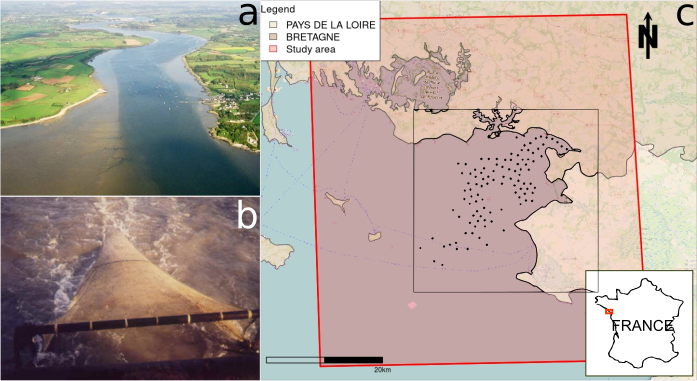
\includegraphics[width=0.8\linewidth]{/mnt/Data/ThinkR/Gitlab/formation-glm/03_Figures/00_Presentation/Vilaine_Campaign} 

}

\caption{(a) L'estuaire de la Vilaine. (b) Chalut à
perche. (c) Situation des stations d'échantillonnage.}\label{fig:figVilaineCampaign}
\end{figure}

\subsection{Covariables}\label{covariables}

\begin{itemize}
\tightlist
\item
  Bathymétrie (Fig. \ref{fig:figCovariates}a)

  \begin{itemize}
  \tightlist
  \item
    MNT à 1000m de résolution
  \item
    Projection Mercator
  \end{itemize}
\item
  Structure sédimentainre (Fig. \ref{fig:figCovariates}b)

  \begin{itemize}
  \tightlist
  \item
    Fichier shape de polygones
  \item
    Coordonnées géographiques
  \end{itemize}
\item
  Zones biologiques (Fig. \ref{fig:figCovariates}c)

  \begin{itemize}
  \tightlist
  \item
    Combinaison bathymétrie, sédiment, habitat
  \item
    Fichier shape de polygones
  \item
    Coordonnées géographiques
  \end{itemize}
\end{itemize}




\begin{figure}[!h]

{\centering 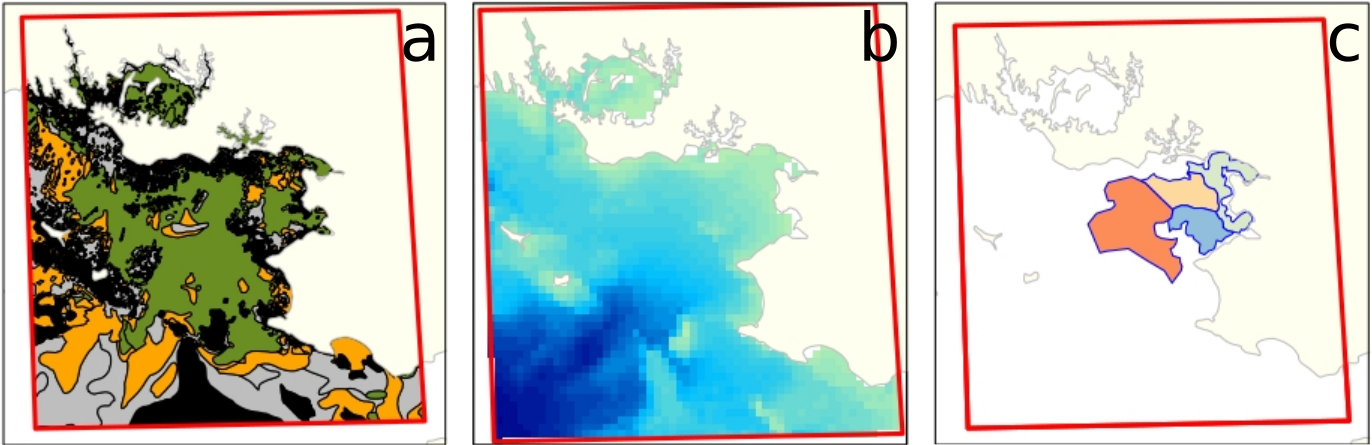
\includegraphics[width=0.8\linewidth]{/mnt/Data/ThinkR/Gitlab/formation-glm/03_Figures/00_Presentation/Day2-02Vilaine-Covariates_abc} 

}

\caption{Covariables en baie de Vilaine. (a) Structure
sédimentaire, (b) Bathymétrie et (c) Zones biologiques.}\label{fig:figCovariates}
\end{figure}

\subsection{Ajuster un modèle de distribution
d'espèces}\label{ajuster-un-modele-de-distribution-despeces}

\begin{itemize}
\tightlist
\item
  Croiser les données avec les cartes de covariables

  \begin{itemize}
  \tightlist
  \item
    Utiliser un modèle linéaire
  \end{itemize}
\item
  Utiliser les cartes des covariables pour la prédiction (Fig.
  \ref{fig:figProcedure})

  \begin{itemize}
  \tightlist
  \item
    Une prédiction pour chaque cellule d'un raster
  \end{itemize}
\end{itemize}



\begin{figure}[!h]

{\centering 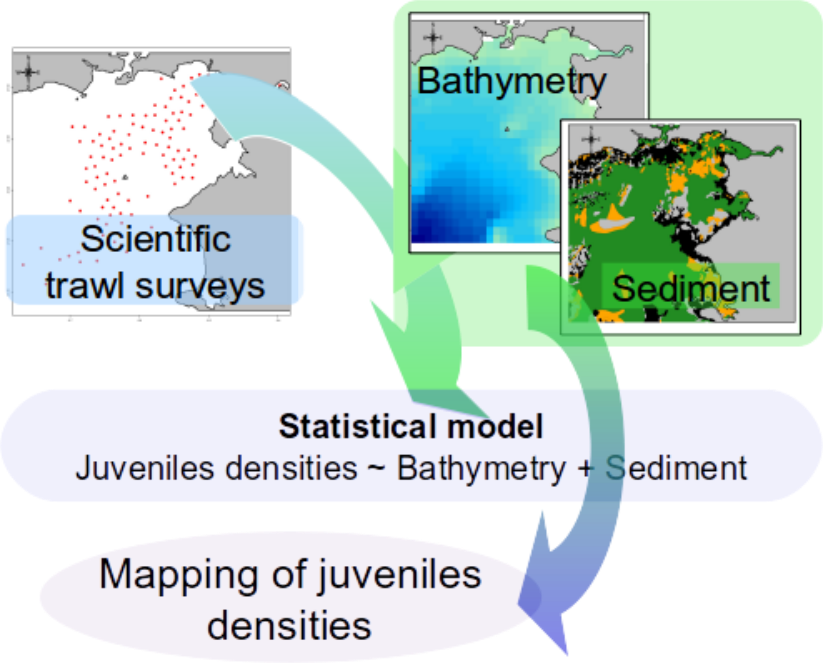
\includegraphics[width=0.7\linewidth]{/mnt/Data/ThinkR/Gitlab/formation-glm/03_Figures/00_Presentation/Schema_Modele} 

}

\caption{Procédure pour un modèle de distribution d'espèce}\label{fig:figProcedure}
\end{figure}

\subsection{Exploration des données}\label{exploration-des-donnees}

\nopandoc{\begin{redbox}} Prenez le temps d'explorer vos données avant
toutes analyses \nopandoc{\end{redbox}}

\begin{itemize}
\tightlist
\item
  Explorer les données et les covariables

  \begin{itemize}
  \tightlist
  \item
    Explorer le plan d'échantillonnage
  \item
    Explorer les liens potentiels entre les densités et les covariables
  \item
    Explorer les futurs paramètres de modélisation (interactions,
    distributions)
  \end{itemize}
\end{itemize}

\advert{Souvenez-vous toujours des objectifs de votre étude !}

\exo{Question : Que recherchons-nous dans cette exploration ?}

\section{Préparation}\label{preparation}

\subsection{Structure des dossiers}\label{structure-des-dossiers}

\advert{Il convient de toujours conserver les fichiers originaux : les reprojections entraînent toujours quelques pertes, mieux vaut revenir aux originaux lorsque c'est possible.}

L'arborescence de votre dossier de travail est la suivante :

\begin{itemize}
\tightlist
\item
  \includegraphics[width=0.26in]{/mnt/Data/ThinkR/Gitlab/vignette-thinkr/img/icon-folder_Blue_12px}
  01\_Original\_data

  \begin{itemize}
  \tightlist
  \item
    \includegraphics[width=0.26in]{/mnt/Data/ThinkR/Gitlab/vignette-thinkr/img/icon-folder_Blue_12px}
    DEPARTEMENTS
  \item
    \includegraphics[width=0.26in]{/mnt/Data/ThinkR/Gitlab/vignette-thinkr/img/icon-folder_Blue_12px}
    Sedim\_GDG\_wgs84
  \item
    \includegraphics[width=0.26in]{/mnt/Data/ThinkR/Gitlab/vignette-thinkr/img/icon-file_Blue_12px}
    bathy\_GDG\_1000\_merc (and co)
  \item
    \includegraphics[width=0.26in]{/mnt/Data/ThinkR/Gitlab/vignette-thinkr/img/icon-file_Blue_12px}
    Data\_Vilaine\_solea.csv
  \end{itemize}
\item
  \includegraphics[width=0.26in]{/mnt/Data/ThinkR/Gitlab/vignette-thinkr/img/icon-folder_Blue_12px}
  02\_Outputs
\item
  \includegraphics[width=0.26in]{/mnt/Data/ThinkR/Gitlab/vignette-thinkr/img/icon-folder_Blue_12px}
  03\_Figures
\item
  \includegraphics[width=0.26in]{/mnt/Data/ThinkR/Gitlab/vignette-thinkr/img/icon-folder_Blue_12px}
  04\_Functions
\end{itemize}

\subsection{Débutons avec R}\label{debutons-avec-r}

\begin{itemize}
\tightlist
\item
  Créer un projet Rstudio dans le dossier principal de travail.
\item
  Ouvrez le script R : ``Quick\_PresAbs\_Student.R''
\item
  Lister les différents sous-dossier de travail au début de votre script
  R
\end{itemize}

\begin{Shaded}
\begin{Highlighting}[]
\CommentTok{# Define working directories ---------------------------------------------------}
\NormalTok{WD <-}\StringTok{ }\KeywordTok{here}\NormalTok{()}
\CommentTok{# Folder of original files}
\NormalTok{origWD <-}\StringTok{ }\KeywordTok{here}\NormalTok{(}\StringTok{"01_Original_data"}\NormalTok{)}
\CommentTok{# Folder for outputs}
\NormalTok{saveWD <-}\StringTok{ }\KeywordTok{here}\NormalTok{(}\StringTok{"02_Outputs"}\NormalTok{)}
\CommentTok{# Folder where to save outputs from R}
\NormalTok{figWD <-}\StringTok{ }\KeywordTok{here}\NormalTok{(}\StringTok{"03_Figures"}\NormalTok{)}
\CommentTok{# Folder where complementary functions are stored}
\NormalTok{funcWD <-}\StringTok{ }\KeywordTok{here}\NormalTok{(}\StringTok{"04_Functions"}\NormalTok{)}
\end{Highlighting}
\end{Shaded}

\subsection{Sous-modèle Binomial}\label{sous-modele-binomial}

\subsubsection{Étapes}\label{etapes}

La procédure à adopter avec le sous-groupe de données est la même
qu'avec le jeu de données complet.

\begin{itemize}
\tightlist
\item
  Créer les observations de présence-absences à partir du jeu de données
\item
  Explorer ce nouveau jeu de données
\item
  Utiliser une distribution binomiale

  \begin{itemize}
  \tightlist
  \item
    Tester les covariables, les interactions, les fonctions de lien, les
    critères de qualité
  \end{itemize}
\item
  Choisir le meilleur modèle
\end{itemize}

\subsubsection{Exploration}\label{exploration}

\subsubsection{Ajuster un modèle binomial avec une fonction de
lien}\label{ajuster-un-modele-binomial-avec-une-fonction-de-lien}

Le choix de la distribution pour un modèle de présence-absence est
simple, c'est un modèle binomial. Cepedant, un modèle est généralement
ajusté sur la base de résidus Gaussiens. Pour ajuster un modèle
binomial, les données doivent être transformées de telle sorte qu'on
puisse ajuster un modèle linéaire Gaussien classique dessus. Pour cela,
nous utilisons une fonction de lien. La fonction de lien classique d'un
modèle binomial est la fonction logit, mais ce n'est pas la seule. Vous
pouvez tester cloglog, probit ou cauchit.

\subsubsection{Qualité d'ajustement d'un modèle
binomial}\label{qualite-dajustement-dun-modele-binomial}

Une mesure couramment utilisée pour la qualité d'ajustement d'un modèle
binomial est ``l'aire sous la courbe'' (AUC : Area Under the Curve). Un
objectif des modèles binomiaux étant de prédire un succès ou un échec,
et non pas seulement une probabilité de succès, on peut vouloir définir
un seuil (intuitivement 0.5 par exemple) qui transforme la probabilité
de présence en présence ou absence. L'AUC est en quelque sorte une
probabilité de classer correctement les présences et absences. Une
définition plus complète serait :

\begin{quote}
La probabililité moyenne pour qu'une observation=1 et une observation=0
choisies de manière aléatoire dans le jeu de données montrent une
probabilité de présence prédite supérieure pour l'observation=1 par
rapport à celle de l'observation=0
\end{quote}

Ainsi, \(AUC = 1\) montrerait un modèle ``parfait'', mais \(AUC = 0.5\)
montrerait un modèle plus mauvais que le hasard.




\begin{figure}[!h]

{\centering 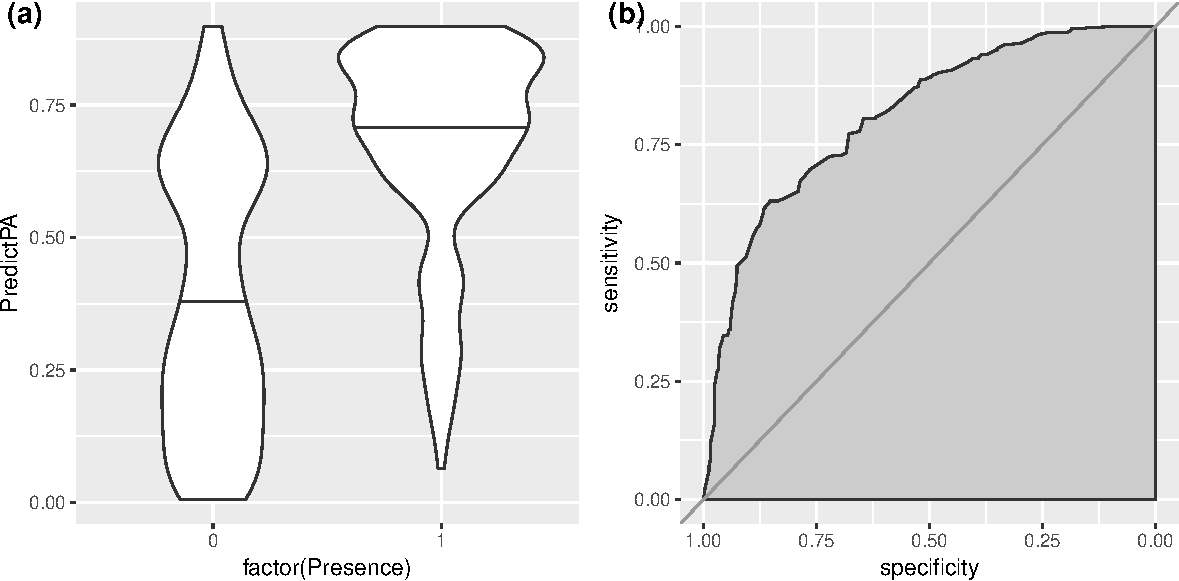
\includegraphics[width=0.9\linewidth]{FR_Quick_PresAbs_Student_files/figure-latex/RFigAUCPA-1} 

}

\caption{(a) Prédiction vs Observations. (b) Courbe ROC d'un
modèle binomial}\label{fig:RFigAUCPA}
\end{figure}

\subsubsection{Choix du meilleur seuil}\label{choix-du-meilleur-seuil}

\begin{itemize}
\tightlist
\item
  \exo{Le modèle sélectionné sur la base de l'AIC est-il toujours le meilleur modèle avec l'AUC sur les données de validation ?}
\end{itemize}


\end{document}
